%------------------------------------------------------------------------------
% CV in Latex
% Author : Charles Rambo
% Based off of: https://github.com/sb2nov/resume and Jake's Resume on Overleaf
% Most recently updated version may be found at https://github.com/fizixmastr 
% License : MIT
%------------------------------------------------------------------------------

\documentclass[A4,11pt]{article}
%\documentclass[letterpaper,11pt]{article} %For use in US
\usepackage{latexsym}
\usepackage[empty]{fullpage}
\usepackage{titlesec}
\usepackage{marvosym}
\usepackage[usenames,dvipsnames]{color}
\usepackage{verbatim}
\usepackage{enumitem}
\usepackage[hidelinks]{hyperref}
\usepackage[english]{babel}
\usepackage{tabularx}
\usepackage{tikz}
\usepackage{fontawesome5}
\usepackage{listings}
\usepackage{xcolor}
\usepackage{enumitem}
\input{glyphtounicode}

\begin{comment}
I am by no means a professional when it comes to the CV's/resumes, I have
received various trainings on how to write a CV and resume from my high 
school, as well as the Austin College and University of Eastern Finland's
career counseling departments. As I intend to share my CV as a template, I 
feel that it is my responsibility to provide explanations of my work.
\end{comment}


%-----FONT OPTIONS-------------------------------------------------------------
\begin{comment}
The font of the document will impact not just how readable it is, but how it is
perceived. In the "The Craft of Scientific Writing" by Michael Alley, shares a
common fonts for publication as well as their use. I have chosen to use
Palatino for its legibility, some others are given below. There is far too much
about typography to discus here. Note: serif fonts have short projecting
strokes, sans-serif fonts are sans (without) these strokes.
\end{comment}


% serif
 \usepackage{palatino}
% \usepackage{times} %This is the default as well
% \usepackage{charter}

% sans-serif
% \usepackage{helvet}
% \usepackage[sfdefault]{noto-sans}
% \usepackage[default]{sourcesanspro}

%-----PAGE SETUP---------------------------------------------------------------

% Adjust margins
\addtolength{\oddsidemargin}{-1cm}
\addtolength{\evensidemargin}{-1cm}
\addtolength{\textwidth}{2cm}
\addtolength{\topmargin}{-1cm}
\addtolength{\textheight}{2cm}

% Margins for US Letter size
%\addtolength{\oddsidemargin}{-0.5in}
%\addtolength{\evensidemargin}{-0.5in}
%\addtolength{\textwidth}{1in}
%\addtolength{\topmargin}{-.5in}
%\addtolength{\textheight}{1.0in}

\urlstyle{same}

\raggedbottom
\raggedright
\setlength{\tabcolsep}{0cm}

% Sections formatting
\titleformat{\section}{
  \vspace{-4pt}\scshape\raggedright\large
}{}{0em}{}[\color{black}\titlerule \vspace{-5pt}]

% Ensure that .pdf is machine readable/ATS parsable
\pdfgentounicode=1

%-----CUSTOM COMMANDS FOR FORMATTING SECTIONS----------------------------------
\newcommand{\CVItem}[1]{
  \item\small{
    {#1 \vspace{-2pt}}
  }
}

\newcommand{\CVSubheading}[4]{
  \vspace{-2pt}\item
    \begin{tabular*}{0.97\textwidth}[t]{l@{\extracolsep{\fill}}r}
      \textbf{#1} & #2 \\
      \small#3 & \small #4 \\
    \end{tabular*}\vspace{-7pt}
}

\newcommand{\CVSubSubheading}[2]{
    \item
    \begin{tabular*}{0.97\textwidth}{l@{\extracolsep{\fill}}r}
      \text{\small#1} & \text{\small #2} \\
    \end{tabular*}\vspace{-7pt}
}

\newcommand{\CVSubItem}[1]{\CVItem{#1}\vspace{-4pt}}

\renewcommand\labelitemii{$\vcenter{\hbox{\tiny$\bullet$}}$}

\newcommand{\CVSubHeadingListStart}{\begin{itemize}[leftmargin=0.5cm, label={}]}
% \newcommand{\resumeSubHeadingListStart}{\begin{itemize}[leftmargin=0.15in, label={}]} % Uncomment for US
\newcommand{\CVSubHeadingListEnd}{\end{itemize}}
\newcommand{\CVItemListStart}{\begin{itemize}}
\newcommand{\CVItemListEnd}{\end{itemize}\vspace{-5pt}}

%------------------------------------------------------------------------------
% CV STARTS HERE  %
%------------------------------------------------------------------------------
\begin{document}

%-----HEADING------------------------------------------------------------------
\begin{comment}
In Europe it is common to include a picture of ones self in the CV. Select
which heading appropriate for the document you are creating.
\end{comment}

\begin{minipage}[c]{0.05\textwidth}
\-\
\end{minipage}
\begin{minipage}[c]{0.2\textwidth}
\begin{tikzpicture}
    \node at (0,-.7) {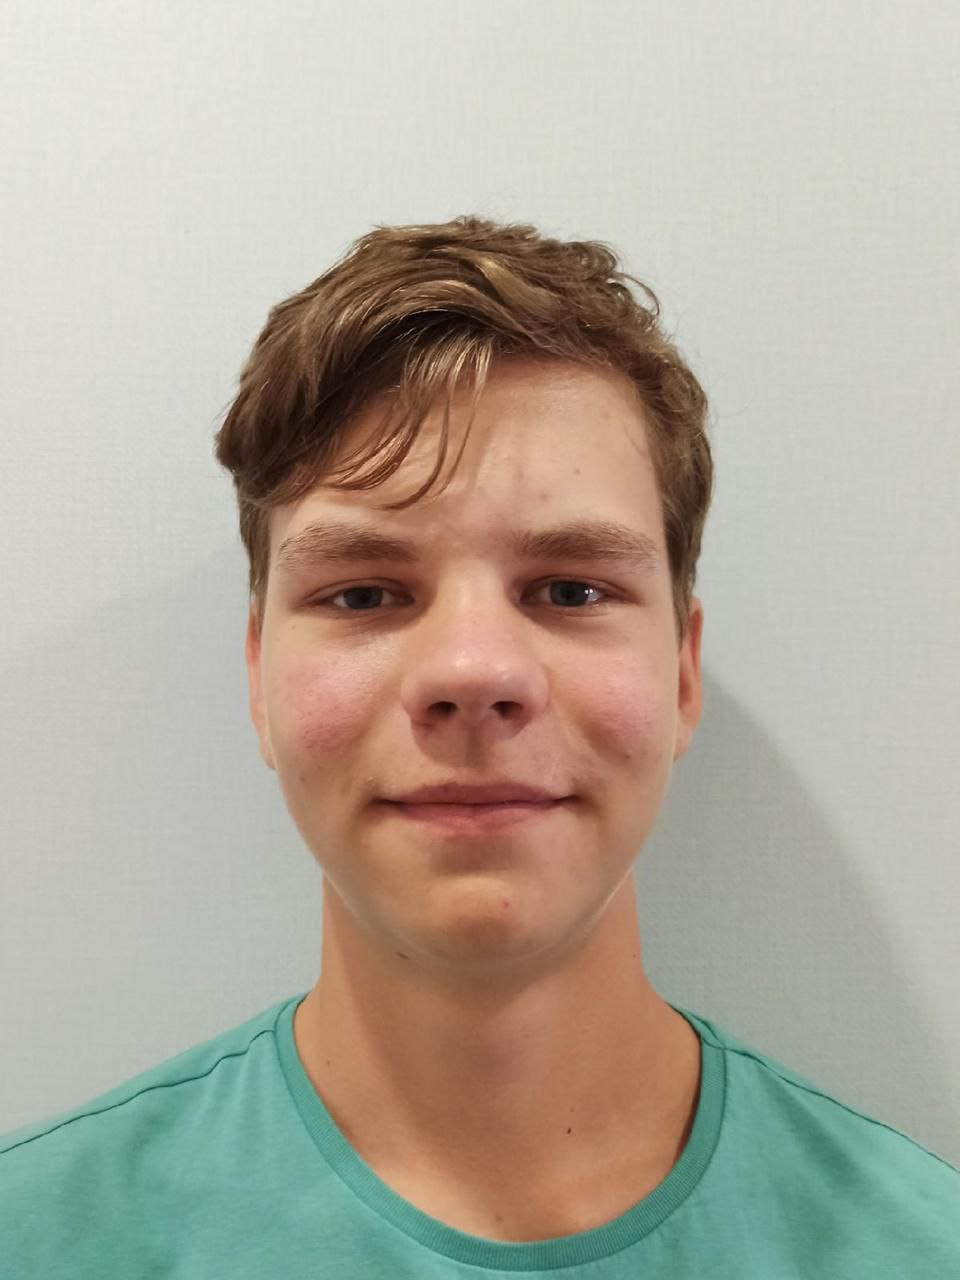
\includegraphics[width = 3cm]{Photo.jpg}}; 
    % if necessary the picture may be moved by changing the at (coordinates)
    % width defines the 'zoom' of the picture
\end{tikzpicture}
\hfill\vline\hfill
\end{minipage}
\begin{minipage}[c]{0.5\textwidth}
    \textbf{\Huge \scshape{Denis Melnikov}} \\  
    % \scshape sets small capital letters, remove if desired
    \small{\faPhone} \hspace{0.1cm} \small{+7 931 511 58 76} \\
    \faEnvelope \hspace{0.1cm} \href{melnikov.denis@phystech.edu}{\underline{melnikov.denis@phystech.edu}}\\
    \faTelegram \hspace{0.1cm} \href{https://t.me/daikofnetu} {\underline{@daikofnetu}} \\
    % Be sure to use a professional *personal* email address
    \faGithub \hspace{0.1cm} \href{https://www.github.com/dinichthys}{\underline{Dinichthys}} \\
    % you should adjust you linked in profile name to be professional and recognizable
    \faMapMarker \hspace{0.1cm} {\underline{Moscow, Russia}} \\
\end{minipage}

% Without picture
%\begin{center}
%    \textbf{\Huge \scshape Charles Rambo} \\ \vspace{1pt} %\scshape sets small capital letters, remove if desired
%    \small +1 123-456-7890 $|$ 
%    \href{mailto:you@provider.com}{\underline{you@provider.com}} $|$\\
%    % Be sure to use a professional *personal* email address
%    \href{https://linkedin.com/in/your-name-here}{\underline{linkedin.com/in/charles-rambo}} $|$
%    % you should adjust you linked in profile name to be professional and recognizable
%    \href{https://github.com/fizixmastr}{\underline{github.com/fizixmastr}}
%\end{center}



\begin{comment}
This CV was written for specifically for positions I was applying for in
academia, and then modified to be a template.

A standard CV is about two pages long where as a resume in the US is one page.
sections can be added and removed here with this in mind. In my experience, 
education, and applicable work experience and skills are the most import things
to include on a resume. For a CV the Europass CV suggests the categories: Work
Experience, Education and Training, Language Skills, Digital Skills,
Communication and Interpersonal Skills, Conferences and Seminars, Creative Works
Driver's License, Hobbies and Interests, Honors and Awards, Management and
Leadership Skills, Networks and Memberships, Organizational Skills, Projects,
Publications, Recommendations, Social and Political Activities, Volunteering.

Your goal is to convey a who, what , when, where, why for every item you share. 
The who is obviously you, but I believe the rest should be done in that order.
For example below. An employer cares most about the degree held and typically 
less about the institution or where it is located (This is still good 
information though). Whatever order you choose be consistent throughout.
\end{comment}

%-----EDUCATION----------------------------------------------------------------
\section{Education}
  \CVSubHeadingListStart
%    \CVSubheading % Example
%      {Degree Achieved}{Years of Study}
%      {Institution of Study}{Where it is located}
    \CVSubheading
      {{Bachelor $|$ \emph{\small{First course, GPA: 8.43}}}}{Sep. 2024 -- Present}
      {Phystech School of Radio Engineering and Computer Technology \\ Moscow Institute of Physics and Technology}{Dolgoprudny, Russia}
  \CVSubHeadingListEnd

% %-----WORK EXPERIENCE----------------------------------------------------------
% \begin{comment}
% try to briefly explain what you did and why it is relevant to the position you
% are seeking
% \end{comment}

% \section{Work Experience}
%   \CVSubHeadingListStart
% %    \CVSubheading %Example
% %      {What you did}{When you worked there}
% %      {Who you worked for}{Where they are located}
% %      \CVItemListStart
% %        \CVItem{Why it is important to this employer}
% %      \CVItemListEnd
%     \CVSubheading
%       {Integration Engineering Intern}{June 2018 -- August 2019}
%       {Finisar Corp.}{Sherman, TX}
%       \CVItemListStart
%         \CVItem{Worked in ISO 4 cleanroom developing applications to improve efficiency and creating specs}
%         \CVItem{Employed metrology and microscopy for failure analysis and developing process for wet etching}
%         \CVItem{Member of Emergency Response Team}
%       \CVItemListEnd
%     \CVSubheading
%       {Laboratory Assistant}{January 2016 -- July 2016}
%       {North Lake College}{Irving, TX}
%       \CVItemListStart
%         \CVItem{Inventoried and maintained Physics Department lab equipment}
%         \CVItem{Physics tutoring}
%     \CVItemListEnd
%     \CVSubheading
%       {Assistant Manager}{December 2006 -- August 2015}
%       {Sun \& Ski Sports}{Austin, TX}
%       \CVItemListStart
%         \CVItem{Led a team of 20+ employees}
%         \CVItem{Ran social media, as well as all grassroots marketing}
%       \CVItemListEnd
%   \CVSubHeadingListEnd

%-----PROJECTS AND RESEARCH----------------------------------------------------
\begin{comment}
Ideally the title of the work should speak for what it is. However if you feel
like you should explain more about why the project is applicable to this job,
use item list as is shown in the work experience section.
\end{comment}
%  Stack
%  Mandelbrot
%  CrackMe
\section{Projects}
  \CVSubHeadingListStart
%    \CVSubheading
%      {Title of Work}{When it was done}
%      {Institution you worked with}{unused}
    \CVSubheading
      {{Programming Language} $|$ \emph{\small{C, make}}}{\href{https://github.com/Dinichthys/Language}{Language on GitHub}}{}{}
      \small{
      \textbf{Project Goal:} Implement a compiler for a custom language with its own syntax, targeting a custom architecture. The front-end module uses a recursive descent parser to analyze the program text and construct an AST (Abstract Syntax Tree). Subsequently, the back-end module translates the AST into assembly code. Finally, the assembly code is converted into binary representation, which is executed by the processor from the SPU project.
      }
    \CVSubheading
      {{SPU} $|$ \emph{\small{C, make}}}{\href{https://github.com/Dinichthys/SPU}{SPU on GitHub}}{}{}
      \small{
      \textbf{Project Goal:} Implement a functional processor simulator with three components:
\begin{itemize}[nosep]
  \item \textbf{Assembler:} Translates assembly code to binary representation.
  \item \textbf{Disassembler:} Reverts binary representation to assembly code.
  \item \textbf{Processor:} Executes the binary instructions.
\end{itemize}
}
    \CVSubheading
      {{Printf} $|$ \emph{\small{Assembly (NASM), C, make}}}{\href{https://github.com/Dinichthys/Printf}{Printf on GitHub}}{}{}
      \small{
      \textbf{Project Goal:} Implement a simplified version of the C function \textbf{printf} in assembly, supporting the following format specifiers:
\lstinline|%c|, \lstinline|%s|, \lstinline|%d|, \lstinline|%b|, \lstinline|%o|, \lstinline|%x|, and \lstinline|%f|. 
The parser uses a \textbf{JUMP-table} to efficiently handle specifier letters.\\
\vspace{0.2cm}
\textbf{Additional Features:}
\begin{itemize}[nosep]
    \item \textbf{File output:} Writing formatted text to files
    \item \textbf{Color support:}
    \begin{itemize}[nosep]
        \item For console output: Insertion ANSI escape sequences for colored text
        \item For file output: Usage of HTML-style color tags (e.g., \lstinline|<font color="red">|)
    \end{itemize}
    \item \textbf{Floating-point support:} Handles \lstinline|%f| specifier for floating-point numbers
\end{itemize}

      }
    \CVSubheading
      {{Mandelbrot Set} $|$ \emph{\small{C, CMake}}}{\href{https://github.com/Dinichthys/Mandelbrot}{Mandelbrot Set on GitHub}}{}{}
      \small{
      \textbf{Project Goal:} Try to optimize the work of the program, which draws Mandelbrot Set and makes calculations for every point on the screen. \\
\vspace{0.2cm}
\textbf{There are three methods for optimization:}
\begin{itemize}[nosep]
    \item \textbf{Arrays:} Usage of arrays in a specific way, so the compiler translates the operations with it to SIMD instructions.
    \item \textbf{SIMD Instructions:} Usage of intrinsics will optimize the process because one operation will be used for several data at one moment.
    \item \textbf{Loop unrolling:} Loop unrolling helps to execute data-independent instructions in a parallel way, because the pipeline of the processor will be full filled of instructions, which won't follow to \textbf{bubble} and \textbf{stall}.
\end{itemize}

      }
      \CVSubheading
      {{Stack} $|$ \emph{\small{C, make}}}{\href{https://github.com/Dinichthys/Stack}{Stack on GitHub}}{}{}
      \small{
      \textbf{Project Goal:} Write a data structure \textbf{stack} with several levels of protections:
\begin{itemize}[nosep]
  \item \textbf{Hash Protection:} This level of protection will count a hash of stack's structure and it's elements and compare it with the correct value.
  \item \textbf{Canary Protection:} This level of protection will add the flag-elements before and after stack's structure and array of it's elements to protect it from vulnerabilities such as buffer overflow.
  \item \textbf{Encapsulation:} This level of protection will oblige the user to work with stack only with functions to exclude the possibility of changing the value of stack elements outside of functions.
\end{itemize} 
      }
    \CVSubheading
      {{CrackMe} $|$ \emph{\small{Assembly (TASM), C, make}}}{\href{https://github.com/Dinichthys/CrackMe}{CrackMe on GitHub}}{}{}
      \small{
      \textbf{Project Goal:} Write a program with two vulnerabilities, exchange it with another student and try to crack his program. Also there was a research and comparison of three disassemblers based on the program \textbf{'The Bomb Lab'}:  
\begin{itemize}[nosep]
  \item \textbf{IDA}
  \item \textbf{Radare2}
  \item \textbf{Ghidra}
\end{itemize} 
      }
  \CVSubHeadingListEnd

%-----HONORS AND AWARDS--------------------------------------------------------
\section{Achievements for the previous year}
  \CVSubHeadingListStart
%    \CVSubheading %Example
%      {What}{When}
%      {Short Description}{}
    \CVSubheading
      {Open School Olympiad}{2024}
      {The winner of the Math Olympiad from ITMO university.}{}
    \CVSubheading
      {Interregional Olympiad of schoolchildren named after I.Ya. Verchenko}{2024}
      {Medalist of the Math Olympiad}{}
    \CVSubheading
      {The Formula of Unity}{2024}
      {Medalist of the Physics Olympiad}{}
    \CVSubheading
      {Phystech School Olympiad}{2024}
      {Medalist of the Math Olympiad}{}
    \CVSubheading
      {Rosatom Branch Physics and Mathematics Olympiad for Schoolchildren}{2024}
      {Medalist of the Math Olympiad}{}
    \CVSubheading
      {Rosatom Branch Physics and Mathematics Olympiad for Schoolchildren}{2024}
      {Medalist of the Physics Olympiad}{}
    \CVSubheading
      {Regional stage of the All-Russian School Olympiad}{2024}
      {Medalist of the Informatics Olympiad}{}
    \CVSubheading
      {Regional stage of the All-Russian School Olympiad}{2024}
      {Medalist of the Math Olympiad}{}
    \CVSubheading
      {Regional stage of the All-Russian School Olympiad}{2024}
      {Medalist of the Physics Olympiad}{}
  \CVSubHeadingListEndRegional

%-----INTERESTS-------------------------------------------------------------------
\begin{comment}
This section is compressed from the various skills sections that Euro CV
recommends.
\end{comment}

\section{Interests}
 \begin{itemize}[leftmargin=0.5cm, label={}]
    \small{\item{
     {Profilers}\\
     {Architectures CPU/GPU}\\
     {Compilers}
    }}
 \end{itemize}
    
%------------------------------------------------------------------------------

%-----HARD-SKILLS-------------------------------------------------------------------
\begin{comment}
This section is compressed from the various skills sections that Euro CV
recommends.
\end{comment}

\section{Hard Skills}
 \begin{itemize}[leftmargin=0.5cm, label={}]
    \small{\item{
     \textbf{Programming Languages}{: C, Assembly (NASM, TASM, x86-64), Python} \\
     \textbf{Tools}{: CMake, Make, IDA, Ghidra, Radare2, edb, gdb} \\
     \textbf{Document Creation}{: Microsoft Office, LaTeX, Markdown}
    }}
 \end{itemize}
    
%------------------------------------------------------------------------------

%-----LANGUAGE-------------------------------------------------------------------
\begin{comment}
This section is compressed from the various skills sections that Euro CV
recommends.
\end{comment}

\section{Languages}
 \begin{itemize}[leftmargin=0.5cm, label={}]
    \small{\item{
\textbf{Russian:} Native \\
\textbf{English:} B1
    }}
 \end{itemize}
    
%------------------------------------------------------------------------------

%-----SOFT-SKILLS-------------------------------------------------------------------
\begin{comment}
This section is compressed from the various skills sections that Euro CV
recommends.
\end{comment}

\section{Soft Skills}
 \begin{itemize}[leftmargin=0.5cm, label={}]
    \small{\item{
     {Communication skills}\\
     {Self-confidence}\\
     {Responsibility}
    }}
 \end{itemize}
    
%------------------------------------------------------------------------------

\end{document}